\documentclass[11pt,a4paper]{article}
\usepackage[margin=2.2cm]{geometry}
\usepackage{graphicx,booktabs,xcolor,array}
\usepackage[inline]{enumitem}
\usepackage[hidelinks]{hyperref}
\usepackage{fancyhdr}
\pagestyle{fancy}\fancyhf{}
\lhead{34870 Loudspeaker project -- lab results 10 Nov 2026}\rhead{Group 10, System D}\cfoot{\thepage}
\setlength{\parskip}{4pt}\setlength{\parindent}{0pt}
\newcommand{\good}{\textcolor{green!50!black}{\textbf{good}}}
\newcommand{\fix}{\textcolor{orange!85!black}{\textbf{to fix}}}
\begin{document}

{\LARGE\bfseries Lab day 10 November: results}\\[2pt]
{\large 34870 Electroacoustics, loudspeaker project, Group 10 (System D)}\\[2pt]
{\small Data: \texttt{lab-day/data/} (clean copies) and \texttt{raw data/} (lab-PC files). Figures: \texttt{analysis/results\_labday.m}. Log: \texttt{LOG\_2026-11-10.md}.}

\section*{In one paragraph}
Once the setup was right, the built system does what the design said it would. The woofer and the
mid/tweeter channel are balanced to within 0.1\,dB, the two crossovers are \emph{more} in phase than
the model predicted, and the measurements repeat to within 0.16\,dB half an hour later. The one real
deviation is tonal: the \textbf{tweeter is about 2.7\,dB too quiet} and the midrange about 1.5\,dB too loud
against the model. That widens the on-axis spread from the predicted 4.0\,dB to 7.1\,dB
(150\,Hz--15\,kHz). Changing one resistor fixes most of it: \textbf{Rp 3.3\,$\Omega$ $\rightarrow$
8.2\,$\Omega$} brings the spread down to about 5.3\,dB. This is predicted from our own measurement, not
only from the model.

\begin{center}\small
\begin{tabular}{@{}>{\raggedright}p{6.2cm}>{\raggedright}p{6.6cm}l@{}}\toprule
Quantity & Result & Verdict\\\midrule
On-axis spread 150\,Hz--15\,kHz (1/6 oct) & 7.1\,dB (model 4.0\,dB) & \fix\\
Woofer vs mid+tweeter level & $-0.1$\,dB (after Out 1 $= -10.3$\,dB) & \good\\
Woofer / midrange / tweeter vs model & $-0.1$ / $+1.5$ / $-2.7$\,dB & \fix\ (tweeter)\\
Woofer-flip notch & 315\,Hz, $-32$\,dB (model 329\,Hz, $-21$\,dB) & \good\\
Tweeter-flip notch & 4161\,Hz, $-28.6$\,dB (model 3928\,Hz, $-14$\,dB) & \good\\
Repeat after 31 min (R5 $-$ R1) & median $+0.07$\,dB, worst 0.16\,dB & \good\\
Sum check $|$woofer $+$ mid/tw$|$ vs $|$all$|$ & worst 0.10\,dB & \good\\
Near field at 200\,mm vs Lab D & within 1\,dB over 91\,\% (cone), 86\,\% (vent) & \good\\
Board impedance, 30\textdegree, Lab E placement re-check & not measured / not saved & \fix\\\bottomrule
\end{tabular}
\end{center}

\section{What was measured}
Settings: MiniDSP filters pasted from \texttt{data/dsp/MiniDSP\_*.txt} (LR4, 325\,Hz), \textbf{Out 1 $= -10.3$\,dB}
(design $-4.5$\,dB, then another $-5.8$\,dB to balance this lab's amplifier channels), Out 2 $= 0$\,dB,
amplifier about 45\,\%, placement as in Lab E (mic 2.44\,m, 1.15\,m high), vents plugged. A channel was
muted by pulling its speaker cable at the amplifier.

\begin{center}\small
\begin{tabular}{@{}lll>{\raggedright\arraybackslash}p{6.2cm}@{}}\toprule
Time & Run & Settings in the run & Used?\\\midrule
14:28 & R1 try 1 & woofer / mid+tw / all & no: woofer silent in ``all''\\
15:02 & R1 try 2 & woofer / mid+tw / all & no: woofer 6.4\,dB too loud (Out 1 still $-4.5$)\\
15:17 & \textbf{R1} & woofer / mid+tw / all & \textbf{yes}\\
15:24 & R2 try 1 & mid / tw / all & no: ``all'' not switched in time\\
15:31 & \textbf{R2} & mid / tw / all & \textbf{yes}\\
15:40 & \textbf{R3} & all / woofer inverted / tweeter swapped & \textbf{yes}\\
15:48 & \textbf{R5} & repeat of R1 & \textbf{yes}\\
16:28 & \textbf{NF} & near field, cone and vent, one vent at 200\,mm & \textbf{yes}\\\bottomrule
\end{tabular}
\end{center}
Not measured: R4 (30\textdegree), the impedances Z1--Z4. The Lab E re-check of the bare system was run
but not saved to the stick.

\section{The results}
\begin{figure}[h!]\centering
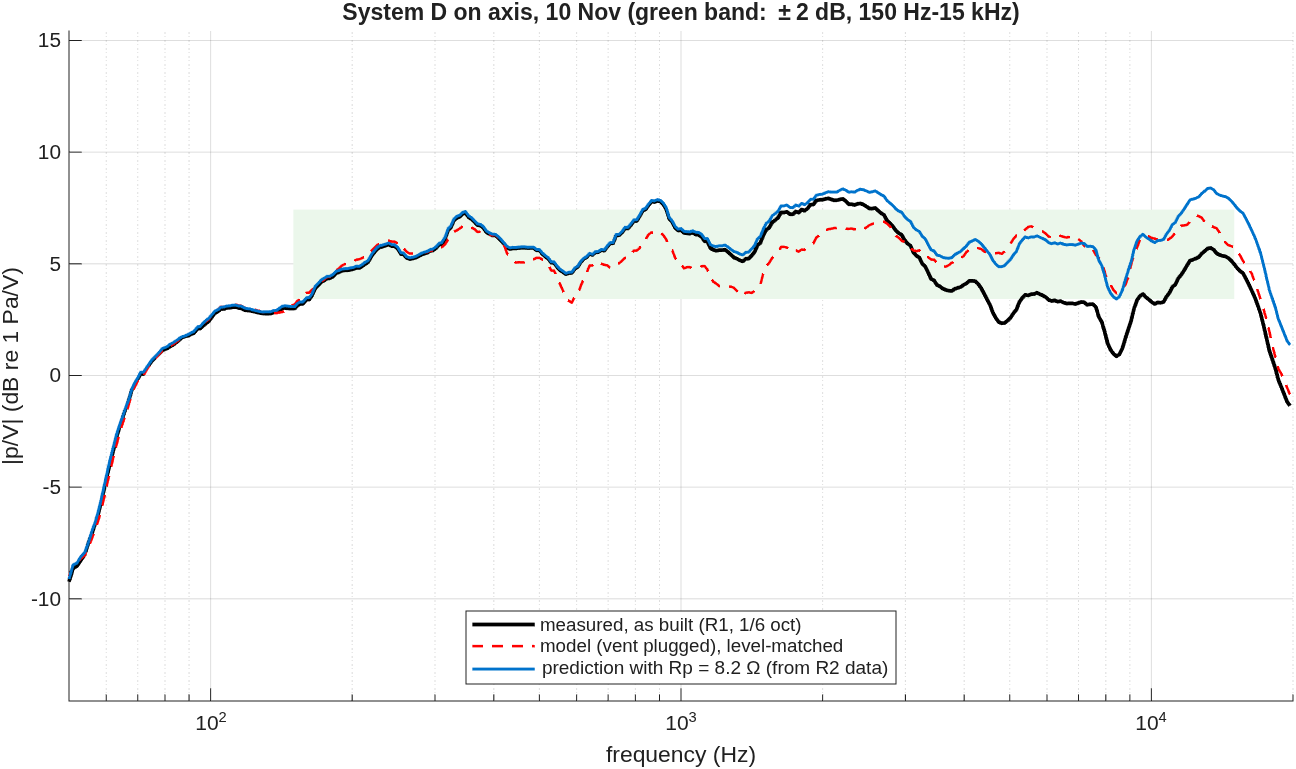
\includegraphics[width=\linewidth]{fig_system.png}
\caption{The whole system on axis. Black: as built. Red dashed: the model (Lab E data through our
filters, vent plugged), shifted to the same level. Blue: what the same measurement becomes with
Rp $= 8.2\,\Omega$ (computed from run R2, see Section~\ref{sec:fix}).}
\label{fig:sys}
\end{figure}

\textbf{Figure~\ref{fig:sys}} is the headline. Up to 3\,kHz the measurement follows the model closely,
with the same ripples at 350\,Hz, 900\,Hz and 2\,kHz. Those ripples come from the drivers and the baffle,
because they are already in the Lab E data. Between 700\,Hz and 3\,kHz we sit about 1.5\,dB above the model;
above 4\,kHz about 3\,dB below it. The 8.3\,kHz dip is in the model too, so it belongs to the tweeter or
the box, not to our crossover.

\begin{figure}[h!]\centering
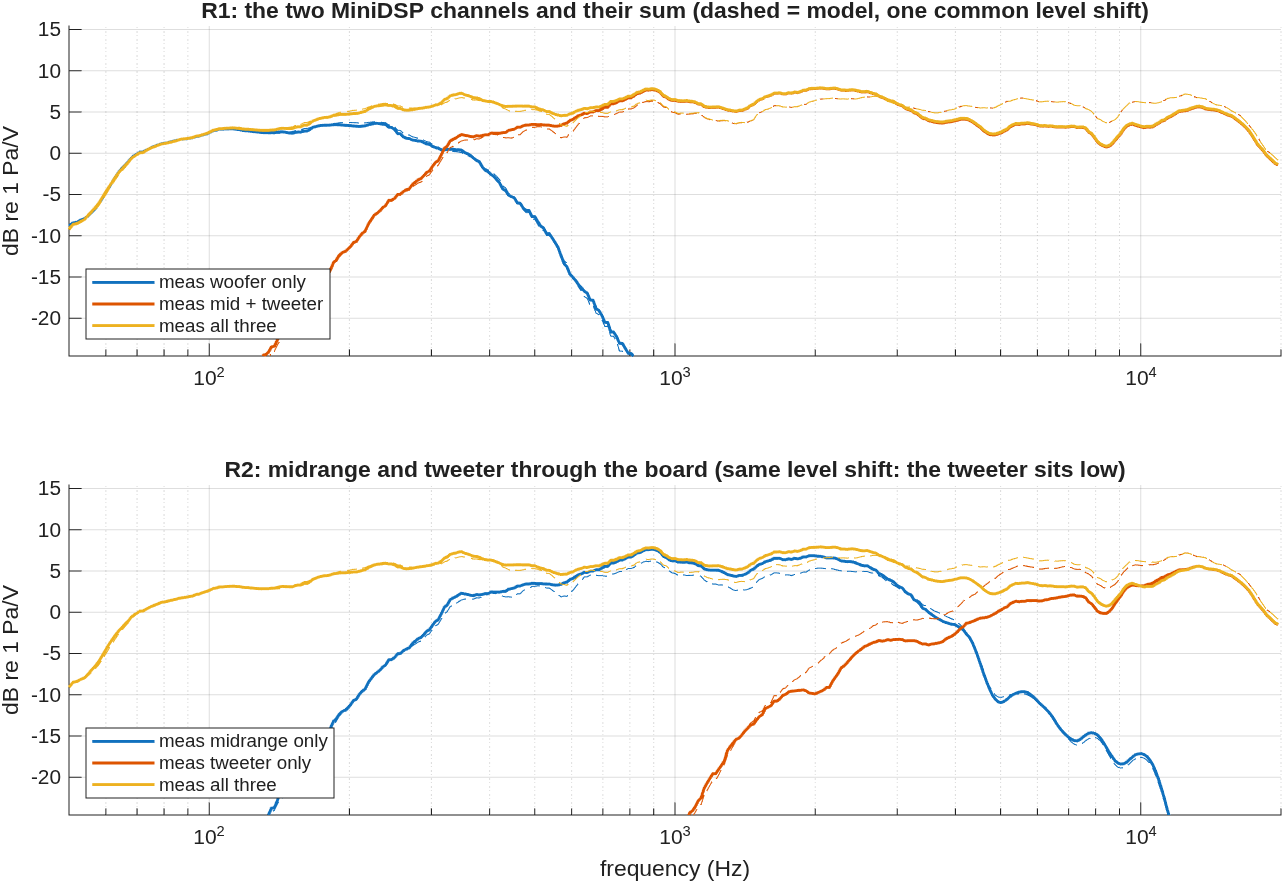
\includegraphics[width=\linewidth]{fig_channels.png}
\caption{Top: the two MiniDSP channels and their sum. Bottom: midrange and tweeter separately through
the board. All dashed model curves are shifted by \emph{one} common amount, so differences in level
between the units are real.}
\label{fig:ch}
\end{figure}

\textbf{Figure~\ref{fig:ch}} shows where that comes from. The woofer lands exactly on its model
($-0.1$\,dB), and the two LR4 slopes cross at the right place and level. In the bottom panel the
midrange runs 1.5\,dB above its model and the tweeter 2.7\,dB below it, so the mid--tweeter balance is
off by about 4\,dB. Three possible causes: the basket resistors and coils are not exactly their nominal
values; the coils' DC resistance (not in the model) lowers the tweeter branch a little; and the tweeter
may simply be less sensitive today than in Lab E. Thursday's placement step P3 (the tweeter through the
board with the MiniDSP bypassed) and P3d (tweeter wired straight to the amplifier) separate these.

\begin{figure}[h!]\centering
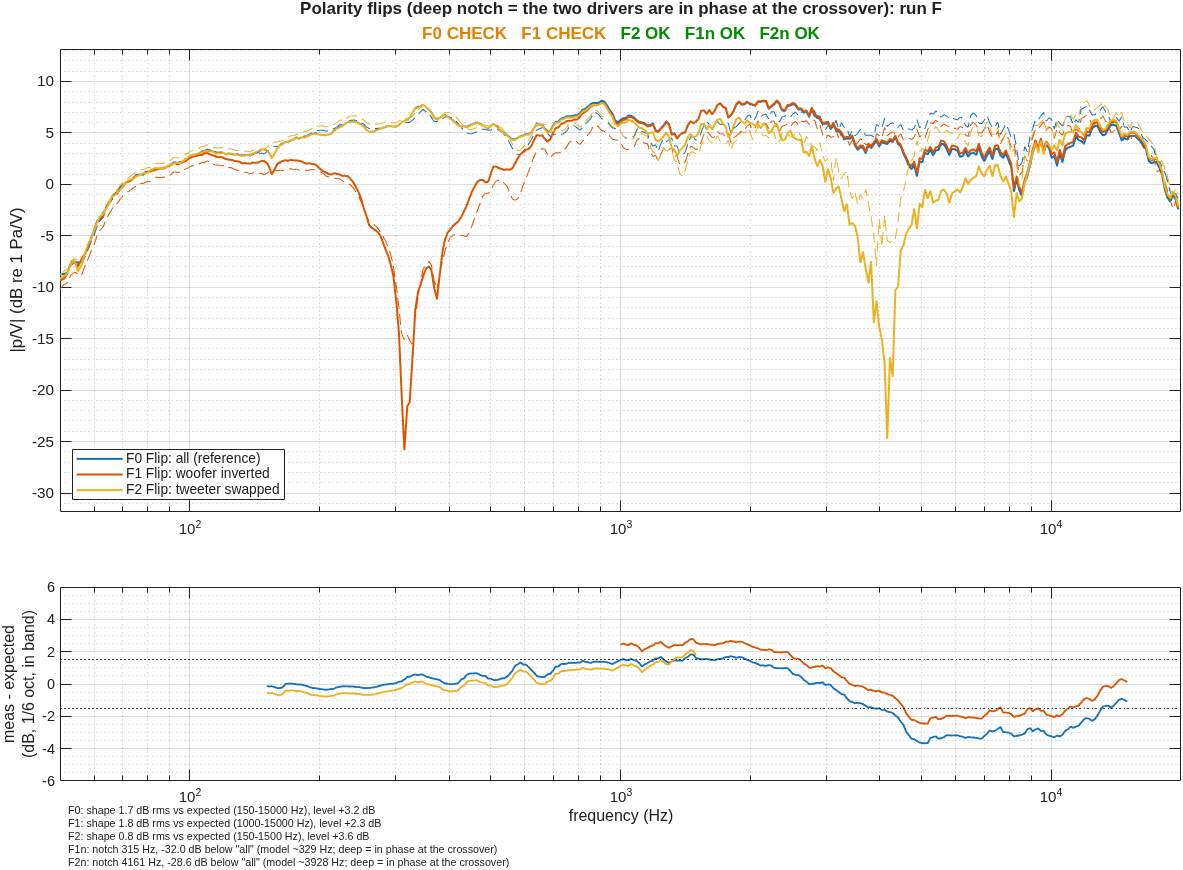
\includegraphics[width=\linewidth]{fig_flips.png}
\caption{Polarity flips (run R3). Inverting one driver turns the sum at the crossover into a
difference; the deeper the notch, the closer the two drivers were to in phase.}
\label{fig:flip}
\end{figure}

\begin{figure}[h!]\centering
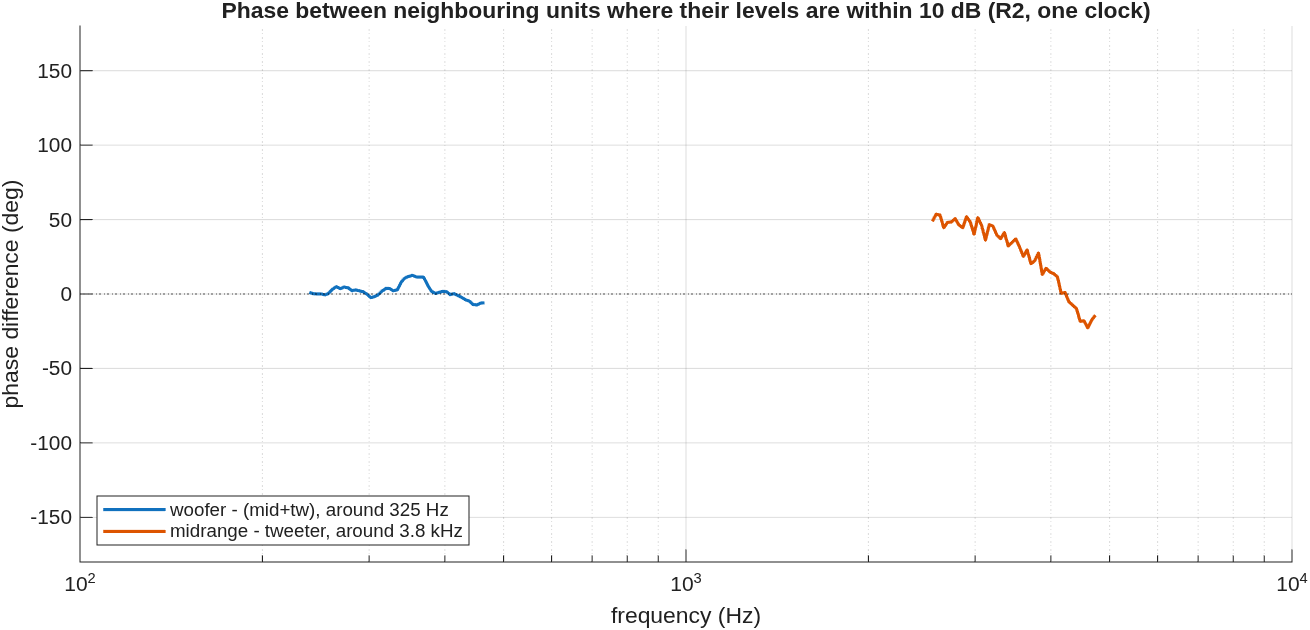
\includegraphics[width=\linewidth]{fig_phase.png}
\caption{Phase difference between neighbouring units, taken from one run (one clock), shown only where
their levels are within 10\,dB of each other.}
\label{fig:phase}
\end{figure}

\textbf{Figures~\ref{fig:flip} and \ref{fig:phase}} test the crossover \emph{integration}. If the drivers
are in phase at the crossover, flipping one of them makes the two cancel, which gives a deep notch. We got
$-32$\,dB at 315\,Hz and $-28.6$\,dB at 4.16\,kHz, deeper than the model's $-21$ and $-14$\,dB. The phase
plot says the same thing directly. Woofer and mid/tweeter stay within about $\pm10$\textdegree\ from 230
to 480\,Hz. Midrange and tweeter go from $+50$\textdegree\ at 2.5\,kHz through 0\textdegree\ at about
4.1\,kHz, which is where the flip notch sits. So in the overlap region the units add up rather than
fight, and there is no hole or peak at either crossover.

\begin{figure}[h!]\centering
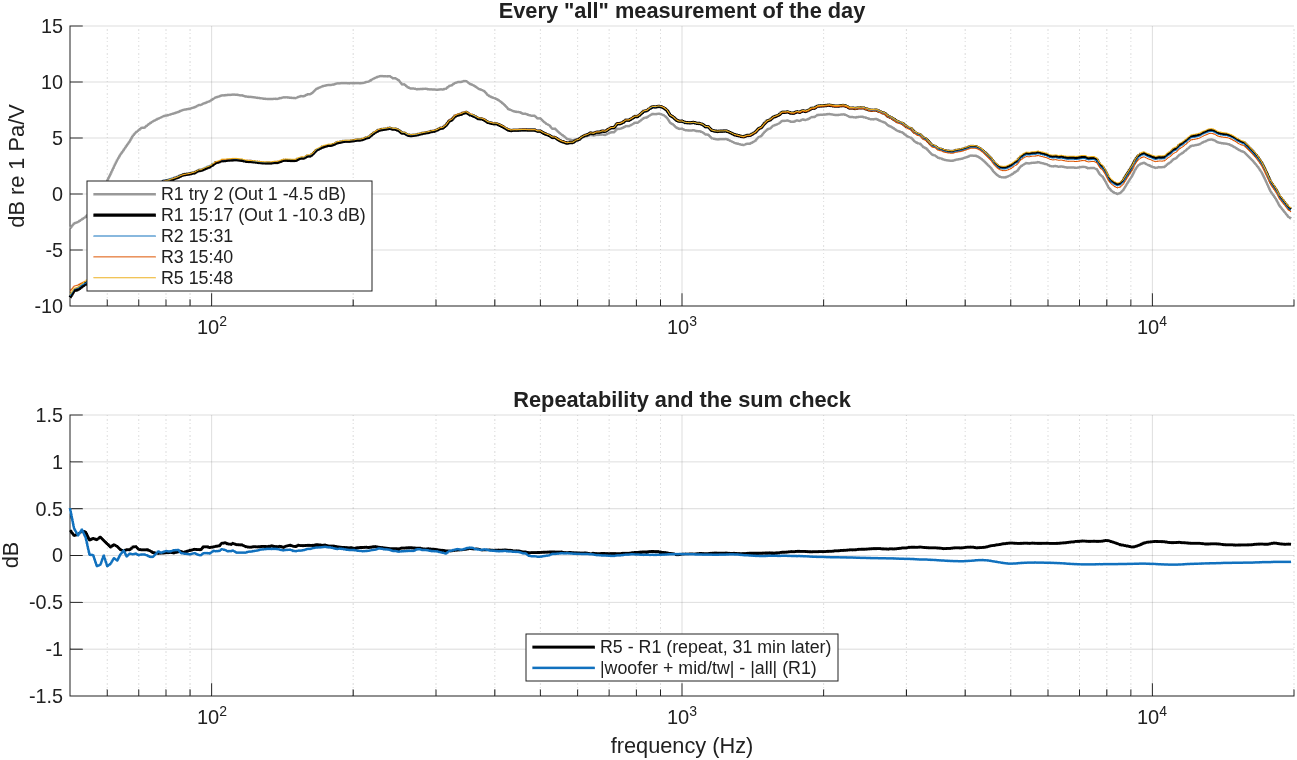
\includegraphics[width=\linewidth]{fig_trust.png}
\caption{Top: every ``all'' measurement of the day. Bottom: the repeat R5 against R1, and the sum check.}
\label{fig:trust}
\end{figure}

\begin{figure}[h!]\centering
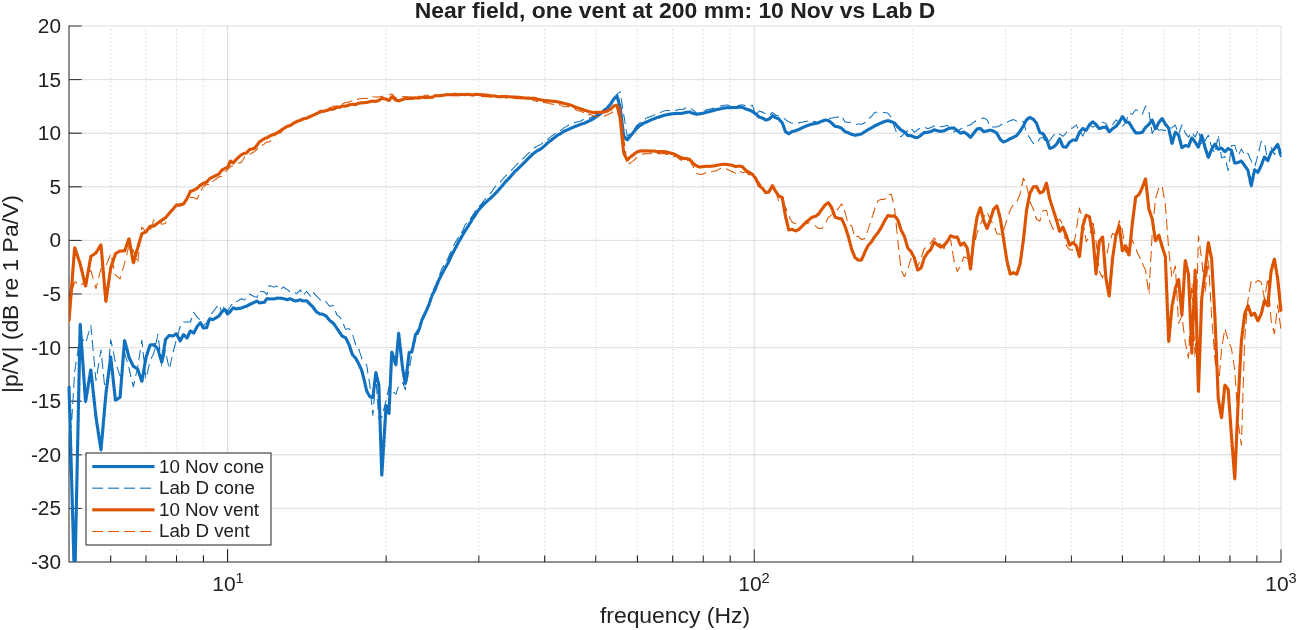
\includegraphics[width=\linewidth]{fig_nearfield.png}
\caption{Near field with one vent at 200\,mm, against the Lab D measurement at the same length.}
\label{fig:nf}
\end{figure}

\section{Why we can trust these measurements}
\begin{itemize}[leftmargin=*]
\item \textbf{They repeat.} R5 was the same measurement as R1, 31 minutes later, after three other runs and a lot of
cable pulling and polarity swapping. It lands within 0.16\,dB everywhere (Figure~\ref{fig:trust}). Nothing
moved and nothing drifted: not the microphone, the temperature or the amplifier.
\item \textbf{They are self-consistent.} Within one run the woofer state plus the mid/tweeter state must
add up, as complex numbers, to the ``all'' state. They do to within 0.10\,dB. That can only happen if the
system is linear, nothing was touched between the states, and the phase reference held.
\item \textbf{They agree with independent earlier data.} The whole shape up to 3\,kHz, including the small
ripples, matches the model built from Lab E. The near field matches Lab D to within 1\,dB over about
90\,\% of 10--200\,Hz (Figure~\ref{fig:nf}). The remaining differences are where the signal is tiny: the
cone's own dip at the vent tuning (21\,Hz), where the vent does the work, and the vent above 190\,Hz.
That also tells us the box (filling, plugs, vent) is the same as in Lab D, so the Lab D 160\,mm data can
still be used for the design.
\item \textbf{The station no longer needs the Lab D correction.} Its input showed no DC offset today, so no factor of 2 was applied.
Its levels still match the Lab D data, where we \emph{did} apply that factor, which confirms the correction was right.
\item \textbf{What we cannot claim yet}: anything off axis (R4 missing), the amplifier load (impedance
not measured), and whether the bare drivers are exactly where they were in Lab E (the Lab E re-check was not saved).
\end{itemize}

\section{What to improve}\label{sec:fix}
\subsection*{The design: one resistor}
The tweeter's level is set by the L-pad: Rs in series and Rp across the tweeter. Run R2 measured mid,
tweeter and ``all'' in one go, so we can take the measured units, change the pad in the board model
only, and add them up again. The result is a prediction made from the real system, not from Lab E.
With Appendix-1 values:
\begin{center}\small
\begin{tabular}{@{}lccc@{}}\toprule
L-pad Rs / Rp ($\Omega$) & tweeter level & spread 150\,Hz--15\,kHz & rms deviation\\\midrule
4.7 / 3.3 (as built) & 0 & 7.2\,dB & 1.64\,dB\\
3.3 / 4.7 & $+2.7$\,dB & 5.6\,dB & 1.34\,dB\\
4.7 / 6.8 & $+2.4$\,dB & 5.3\,dB & 1.21\,dB\\
\textbf{4.7 / 8.2} & $\mathbf{+2.9}$\,dB & \textbf{5.3\,dB} & \textbf{1.20\,dB}\\
3.3 / 6.8 & $+3.8$\,dB & 6.5\,dB & 1.35\,dB\\\bottomrule
\end{tabular}
\end{center}
\textbf{Swap Rp from 3.3 to 8.2\,$\Omega$} and keep everything else. The amplifier still sees at least
4.1\,$\Omega$. The rest of the spread is the 1--3\,kHz region sitting a bit high and the 8.3\,kHz dip. The dip is
in the tweeter's own response, so the crossover cannot remove it. Measure the new board on Thursday
(run S, then S4 + S5) and check that the tweeter step closes.

\subsection*{The procedure}
\begin{itemize}[leftmargin=*]
\item \textbf{Start with the placement check, and save it.} Thursday's kit has it as step P (woofer, mid,
tweeter with the MiniDSP bypassed, each plotted against Lab E).
\item \textbf{A graph after every measurement, with a clear OK/CHECK/BAD.} The new kit (\texttt{lab-day/kit},
\texttt{lab P}, \texttt{lab S}, \dots) does exactly that, plus a dashboard that always shows the whole day.
The same kit has a window, \texttt{labgui}: the steps with lamps, what to set up, one Measure button, the graph, the verdict and what to do next.
\item \textbf{Write the settings down before measuring.} They go in the Settings panel of \texttt{labgui} (or \texttt{lab\_setup.m}): Out 1 gain, amplifier, vent, series R, temperature.
\item \textbf{Save the MiniDSP configuration as a preset}, so the listening test and the demo start from the same state.
\item \textbf{Measure the missing pieces}: board impedance Z1--Z3 (the amplifier load, and the best check of
the board) and 30\textdegree\ (run A).
\item \textbf{Vent at 160\,mm} for listening and the demo. That is the design ($f_B$ 24.6\,Hz). The 200\,mm setting came from a
memory of Lab D, where 200 was simply measured first.
\item \textbf{The IEC room has its own amplifier}: check the woofer/mid balance there before listening
(one run S). The $-10.3$\,dB on Out 1 may not be right in that room.
\end{itemize}

\section{What makes a loudspeaker sound good}
Decades of blind listening tests (Toole, Olive and others at NRC and Harman) agree on a short list. In order of importance:
\begin{enumerate}[leftmargin=*]
\item \textbf{A flat, smooth on-axis response.} This is the timbre: voices and instruments sound like
themselves. Narrow peaks and dips matter less than broad tilts and steps. A 3\,dB shelf over two
octaves, like our tweeter step, is more audible than a sharp 6\,dB notch. That is why the Rp change is worth more than chasing the 8.3\,kHz dip.
\item \textbf{A smooth off-axis response that looks like the on-axis one, only lower.} In a room most
of what reaches you after the first few milliseconds is off-axis sound reflected from the walls. If the
directivity changes abruptly, for example where a large midrange that already beams hands over to a
small tweeter that radiates widely, the reflections get a different colour from the direct sound. That
is our open question at the 3.8\,kHz crossover: the 5\textonequarter'' midrange has $ka \approx 3.5$
there (beaming), while the 25\,mm tweeter has $ka \approx 0.9$ (wide). The 30\textdegree\ run will show how big
the step is. A slightly lower mid/tweeter crossover reduces it, but the tweeter resonance (1.45\,kHz) limits how far down it can go.
\item \textbf{Well-integrated crossovers.} The units must add up in phase where they overlap, or you
get a hole or a bump that also moves with listening height. Ours is good (Figures~\ref{fig:flip}, \ref{fig:phase}).
\item \textbf{Clean, extended bass without boom.} Low-frequency extension (our $f_3$ is about 33\,Hz) is
appreciated, but a peak in the bass (too high a $Q$, or a room mode) is heard as boom and muddiness. The
vent tuning and the room together decide this, so it is judged in the IEC room, not in the anechoic chamber.
\item \textbf{Low distortion and enough level.} This is mostly a property of the drivers and the box. For
us it means not driving the woofer past its excursion limit (X$_\mathrm{max}$ 6\,mm) and keeping the
midrange's high-pass steep enough.
\item \textbf{Balance against the room.} A speaker that is flat on axis and whose directivity rises
smoothly with frequency gives a steady downward tilt in the room, roughly $-1$\,dB/octave. That
in-room slope is what most listeners prefer. So ``flat in the chamber'' is the right first target: the room adds the tilt.
\end{enumerate}

\subsection*{Flat first, then tune: how, within the course rules}
The MiniDSP's PEQ, Comp and FIR blocks must stay bypassed (they cannot be exported to LTspice), so the tools are:
\begin{center}\small
\begin{tabular}{@{}>{\raggedright}p{4.2cm}>{\raggedright}p{5.2cm}p{5.4cm}@{}}\toprule
Knob & What it changes & Typical use\\\midrule
Out 1 gain (woofer) & everything below about 325\,Hz against the rest & bass ``fuller'' $+1$--2\,dB or ``leaner''\tabularnewline
Out 2 gain (mid+tweeter) & the same balance from the other side & keep at 0 and use Out 1\tabularnewline
L-pad Rs/Rp & tweeter level above about 4\,kHz & ``bright'' vs ``dull'': steps of about 1--3\,dB\tabularnewline
MiniDSP crossover frequency & the woofer/mid handover & 300--400\,Hz; the woofer starts beaming above about 500\,Hz\tabularnewline
Passive mid/tweeter values & where the mid hands over, and the shape of the overlap & lower crossover = smoother directivity\tabularnewline
Vent length / filling & bass extension against boom & 160\,mm design; longer = lower $f_B$, less output near 30\,Hz\tabularnewline\bottomrule
\end{tabular}
\end{center}
A workable procedure:
\begin{enumerate*}[label=(\arabic*)]
\item measure until the system is flat (Rp $= 8.2$, check run S);
\item listen in the IEC room with 4--5 familiar tracks and a short questionnaire (balance,
brightness, bass, clarity, imaging; 1--5 scale);
\item change \emph{one} knob by 1--2\,dB, listen again blind if possible (one person switches);
\item measure whatever you keep, so the report shows what ``sounds good'' means as a curve.
\end{enumerate*}

\section{Thursday}
\begin{enumerate}[leftmargin=*]
\item In MATLAB: \texttt{cd lab-day/kit}, type \texttt{labgui}. Fill in Settings (Out 1 $-10.3$\,dB, amplifier, vent 160\,mm, series R). The steps below are the entries in its list; \texttt{lab P} etc.\ typed in the command window, or the sections of \texttt{lab\_run.m}, do the same.
\item \texttt{lab P}: placement against Lab E. All three should be OK before going on.
\item Put \textbf{Rp $= 8.2\,\Omega$} on the board. \texttt{lab S}, \texttt{lab S4}, \texttt{lab S5}: check the tweeter step is gone and the balance is still within $\pm1$\,dB.
\item \texttt{lab F}, \texttt{lab A} (30\textdegree), and at the Zi station \texttt{lab Z1}--\texttt{Z4}, \texttt{lab N1}, \texttt{N2}.
\item The dashboard shows everything as you go. Copy \texttt{data/<date>/} (including its \texttt{figures/}) to the stick.
\end{enumerate}
\end{document}
